\documentclass[projekt,german]{hgbthesis}
% Zulässige Class Options: 
%   Typ der Arbeit: diplom, master (default), bachelor, praktikum 
%   Hauptsprache: german (default), english
%%------------------------------------------------------------

%Zeilenabstand anpassen
%\usepackage[onehalfspacing]{setspace}

%\usepackage[doublespacing]{setspace}

\graphicspath{{images/}}    % wo liegen die Bilder? 
%\addbibresource{literatur.bib}  	% Angabe der BibTeX-Datei, % utf8-change
\bibliography{literatur.bib}


%%%----------------------------------------------------------
\begin{document}
%%%----------------------------------------------------------

% Einträge für ALLE Arbeiten: --------------------------------
\title{Anzeigetafel für ein Fußballspiel}
\author{Daniel H.\ Vogt und Lukas Feltes}
\studiengang{Angewandte Informatik}
\studienort{Karlsruhe}
\studienuni{DHBW Karlsruhe}
\abgabedatum{2018}{06}{14}	% {YYYY}{MM}{DD}
 
\semester{Sommersemester 2018}  
 
\nummer{9552394 und 9584715}    
 

\cclicense

%\strictlicense  % erzeugt restriktive Lizenzformel

%%%----------------------------------------------------------

\frontmatter
\maketitle
\tableofcontents
%%%----------------------------------------------------------

%\include{kurzfassung}		
%\include{abstract}			

%%%----------------------------------------------------------
\mainmatter         % Hauptteil (ab hier arab. Seitenzahlen)
%%%----------------------------------------------------------

\chapter{Einleitung}
\label{cha:Einleitung}


\section{Motivation}
Dieses Projekt findet im Rahmen der Vorlesung Systemnahe Programmierung an der Dualen Hochschule Baden-Württemberg statt. Ziel dieser Vorlesung ist es Kenntnisse über die systemnahe Programmierung zu vermitteln und so das Schreiben systemnaher Programme zu lernen. Innerhalb der Vorlesung wird Assembler für die 8051 Mikrokontroller verwendet. Um die erlernten Grundlagen dieser Vorlesung auch praktisch einsetzen zu können, wird ein Projekt erstellt und in einer virtuellen Entwicklungsumgebung ausgeführt. Dafür wurde die MCU-8051 IDE verwendet.  

Bei der Gestaltung des Projektes können die Studenten eigene Ideen umsetzen. Aufgrund unserer eigenen großen Sportleidenschaft haben wir uns dafür entschieden eine Fußballanzeigetafel mit Spielstand und Zeitanzeige zu implementieren. 


\section{Aufgabenstellung}
Die zu implementierende Anzeigetafel sollte sowohl den aktuellen Spielstand, sowie die bereits gespielte Zeit anzeigen (siehe Abb. \ref{fig:Anzeigetafel}). Dabei soll die Zahl der erzielten Tore oder Punkte über angeschlossene  Knöpfe steuerbar sein. Optional zu diesen Implementierungen soll zusätzlich eine Hupe die bei Ablauf der Spielzeit ertönt implementiert werden. Der aktuelle Spielstand und die Zeit soll per Knopfdruck zurück setzbar sein. 

Für die Implementierung der Anzeigetafel werden nur die innerhalb der Entwicklungsumgebung vorgegebenen Hilfsmittel genutzt. 

\begin{figure}[h]
	\centering
	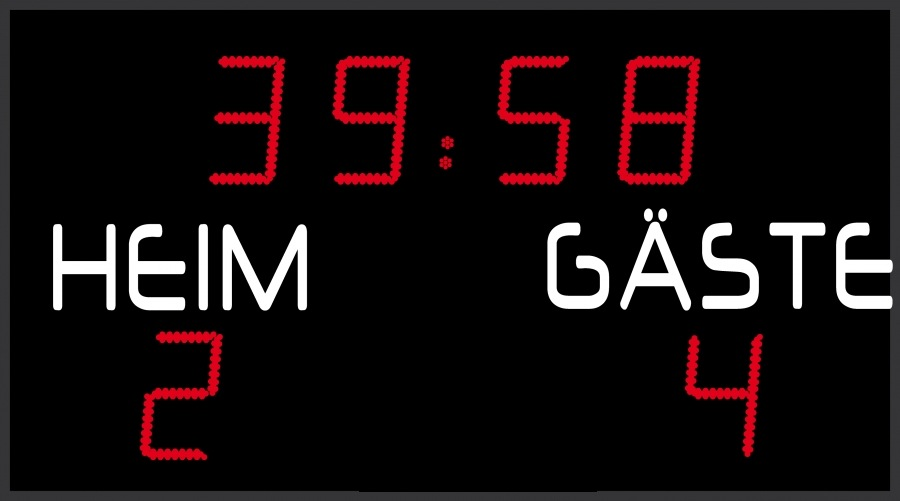
\includegraphics[width=0.9\textwidth]{Anzeigetafel} 
	\caption{Abbildung Anzeigetafel  https://pimage.sport-thieme.de/detail-fillscale-min-height/stramatel-anzeigetafel-ffbffc/131-5400 }
	\label{fig:Anzeigetafel}
\end{figure}		% ggfs. weglassen
\chapter{Grundlagen} 
\label{cha:Grundlagen}
 
 \section{Assembler} 
Der erste bekannte Assembler wurde zwischen 1948 und 1950 geschrieben.

Eine Assemblersprache, kurz auch Assembler genannt, ist eine Programmiersprache, die auf den Befehlssatz einer bestimmten Prozessorarchitektur ausgerichtet ist. Assemblersprachen  sind maschinenorientierte Programmiersprachen. Anstelle eines schwer verständlichen Binärcodes der Maschinensprache können Befehle durch verständliche Symbole in Textform dargestellt werden. Zur Übersetzung eines Assemblerprogramms in Maschinencode wird eine Übersetzungssoftware genutzt. Der Quelltext in Assemblersprache wird auch als Assemblercode bezeichnet.

Die verschiedenen Computerarchitekturen nutzen dabei eigene Maschinensprachen und damit auch eigene Assemblersprachen. Diese Sprachen unterscheiden sich der verschiedenen Architekturen in Anzahl und Typ der Operationen. Jedoch haben alle Architekturen dieselben grundlegenden Operationen. \cite{Assemblersprache}   
 
 \section{Der 8051 Mikrocontroller} 
 
 Die \textbf{8051}-Familie der Mikrocontroller ist eine Prozessorarchitektur von Intel. Sie ist mittlerweile im Originalen veraltet, aber es gibt weitere Varianten, die teilweise durchaus auf aktuellem Stand sind. 
 
 Der 8051 ist ein Mikrocontroller bei dem Befehls- und Datenspeicher logisch getrennt sind, auch wenn diese über einen einzigen Bus adressiert werden. Ob es sich dabei um eine Harvard oder eine von Neumann-Architektur handelt, ist umstritten.\cite{8051}
 
Ein paar der verwendeten Befehle des 8051 Befehlssatzes sind folgende: 
 
 \begin{GenericCode}
 mov A, R7	;Register in Akku laden
 mov R0, A	;Akku in Register laden
 setb C		;Set C - for demo purpose	
 JB 042d, bc2	;springe bei gesetzer BAdr
 jmp @A+DPTR	;Brechneter jump
 ret		;reti for interrupt
 	
 \end{GenericCode}
 \cite{Befehlssatz}
 
  
 
 \section{Entwicklungsumgebung MCU-8051 IDE} 
 
 In Zeiten von Emacs, Vim (und Intellij) ist es schwer sich in eine IDE einzufinden, welche viele Bugs hat und langsam arbeitet. 
 Glücklicherweise ist man nicht gezwungen in dieser IDE zu programmieren. Es reicht wenn man dieses Werkzeug nur zum Compilieren und Simulieren nutzt. 
 
 Der Editor dieser IDE unterstützt einen nur sehr wenig beim entwickeln. 
 Die Autovervollständigung ist mangelhaft, da Symbole teilweise nicht gefunden werden. Die Vorschläge für die Vervollständigung erfolgen oft ohne den Kontext oder sind unzureichend vollständig. 
 
 Das Laden und Erstellen von virtueller Hardware ist zu kompliziert und langsam. Die virtuelle Hardware ist mit Abstand das langsamste an der IDE. Konkurrenzprodukte sind um ein Mehrfaches schneller. Komplexe Programme lassen sich damit nur langsam simulieren, große Timer-Intervalle sind zu vermeiden (da es Tage dauern könnte, bis es zu einem Ereignis kommen könnte).
 Der "'Fade out Intervall"` der virtuellen Hardware ist unberechenbar und unabhängig von der Ausfuhrgeschwindigkeit und somit nicht sehr realitätsnah.  
 
 Gut an der IDE sind die gut strukturieren Anzeigen. So lassen sich schnell die Registerinhalte und andere relevante Hardwareinformation auf einen Blick erkennen. Auch die Möglichkeit das Programm Schrittweise oder auch rückwärts ablaufen zu lassen ist hilfreich.
 
 
 
 
 
 
 
 
 
 

\chapter{Konzept} 	% engl. Preface


\section{Analyse}

Zu Beginn des Spiels muss die Zeitanzeige auf null gesetzt werden, also 00:00 anzeigen. Auch die Anzeige für den Spielstand muss null zu null gesetzt werden. Das Spiel und somit der Ablauf der Zeit soll dann per Knopfdruck gestartet werden. Die aktuelle Zeit sowie der Spielstand sollten dabei stets im Hauptspeicher hinterlegt sein. Neben der Option das Spiel per Knopfdruck zu starten, soll man die Zeit anhalten können. Zudem können beide Anzeigen zurück auf 0 gesetzt werden. Auch das Zählen der Tore ist über die Steuerung möglich. Dabei kann die Zahl der Tore sowohl um eins erhöht als auch um eins erniedrigt werden. 

Zur Anzeige der Zahlenwerte dienen 7 Segment Anzeigen. Diese dienen jeweils als Pärchen als verschiedene Anzeigen. Die Aufgaben eines Pärchens ist einmal Anzeigen eines Spielstandes oder das anzeigen der aktuellen Zeit.

Zur Steuerung wird ein Simple Keypad genutzt. Dieses hat acht Knöpfe, die jeweils mit den oben beschriebenen Funktionen belegt werden und so die Anzeigen steuern können.

\begin{figure}[h]
	\centering
	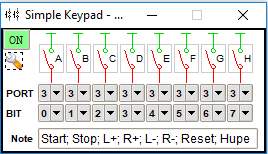
\includegraphics[width=0.9\textwidth]{Button} 
	\caption{Abbildung Simple Keypad  Eigener Screenshot }
	\label{fig:Button}
\end{figure}

\begin{figure}[h]
	\centering
	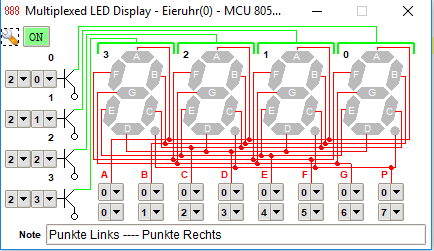
\includegraphics[width=0.9\textwidth]{Spielstand} 
	\caption{Abbildung Spielstand  Eigener Screenshot }
	\label{fig:Spielstand}
\end{figure}

\begin{figure}[h]
	\centering
	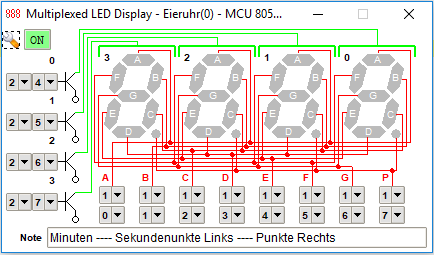
\includegraphics[width=0.9\textwidth]{Zeit} 
	\caption{Abbildung Spielzeit  Eigener Screenshot }
	\label{fig:Zeit}
\end{figure}

\section{Programmentwurf}

Die Ergebnisse der Analyse sollen nun in einen Programmentwurf umgesetzt werden. Zu Beginn werden dafür den verschiedenen Elementen, der in der Analyse beschrieben Hilfsmittel, bestimmte Speicherbereiche zugewiesen.
\begin{table}[H]
	\centering
	\caption{My caption}
	\label{my-label}
	\begin{tabular}{lll}
		Speicheradressbereich & Inhalt  \\
		60h-63h & Punkte  \\
		64h-67h & Zeit   \\
		2Fh & Funktionen  
	\end{tabular}
\end{table}

Neben der Festlegung der Speicherbereiche, wird die Hardware über die I/O Ports verbunden. Dabei werden die folgenden Ports für die jeweiligen Anzeigen genutzt:
\begin{itemize}
	\item Minuten und Sekunden anzeige für ein Fußballspiel (Port0)
	\item Punkte Anzeige für jedes Team  (Port1)
	\item Ansteuerung der jeweiligen 7 Segmentanzeige (Port2)
	\item Simple Keypad zur Steuerung (Port3)
\end{itemize}  


Wenn das Programm aufgerufen wird, kann der Ablauf der Zeit mit dem Simple Keypad eingeleitet werden. Dafür muss der erste Knopf auf dem Keypad einmal gedrückt werden. Er wird somit geschaltet und nimmt den Wert 0 an. Anschließend muss er noch einmal betätigt werden, um die Zeit zu starten, da nur beim Schalten von 0 auf 1 eine Veränderung des Wertes festgestellt wird. Das gleiche gilt für die anderen Knöpfe des Keypads. Auch sie müssen je von 0 auf 1 geändert werden um eine Veränderung zu bekommen. 

Um das Hochzählen der Zeit genau kontrollieren zu können wird ein Timer implementiert der während dem Ablauf des Programmes automatisch hochzählt. Die Zahl wie oft der Timer hochzählt, ist dabei so gewählt, dass genau eine Sekunde vergeht bevor die Anzeige noch einmal hochzählt. Dieser Wert ist aufgrund der Geschwindigkeit der IDE bei unserem Programm kleiner gewählt. 

Das Hauptprogramm läuft eigentlich unabhängig vom Timer selbst. Allerdings kommt es sobald der Timer fertig hochgezählt hat, es also zu einem Überlauf kommt, zu einem Interrupt, durch den das Programm unterbrochen wird. Erst nachdem dieser Interrupt vom Timer beendet wird, kann das Programm weiterlaufen. 

 
 
 
\chapter{Implementation}
\label{cha:Implementation}


Im folgenden Kapitel wird die Implementation des Programmes beschrieben. Da eine komplette Beschreibung des Codes den Rahmen sprengen würde, werden hier nur ausgewählte Abschnitte des Programmes beschrieben.

Zu Beginn des Programmes werden die beschrieben Speicheradressen festgelegt und den Variablen Werte zugewiesen. Im Anschluss daran wird der Timer initialisiert.

Zu Beginn des Ablauf des Hauptprogrammes werden alle Zahlen der 7 Segmentanzeigen neu gezeichnet. Dieses Zeichnen wird im Folgenden genauer beschrieben. 
\label{code:methode}
 \begin{GenericCode}
zeigeAlleSemente: 
push 00h	;Sichere R0
push 01h	;Sichere R1	
push 02h	;Sichere R2	
mov R0, #00d	;aktuelles segment
mov R1, #00d	;Pointer für wert von segment

mov A, #01d
cpl A
mov R2, A	;selectiertes segment... wird rotiert

;clear all 7segs 
mov P2, #00h
mov P0, #0FFh
mov P1, #0FFh
mov P2, #0FFh 

loopAlleSegmente:
CJNE R0, #08d, doFuerSegment     ;für alle 8 segmente
pop 02h		;Wiederherstellen von R2
pop 01h		;Wiederherstellen von R1
pop 00h		;Wiederherstellen von R0
ret

doFuerSegment:
;	Lade Segment mit entsprechendem Wert
mov p2, R2	;aktivate segment mit P2



mov A, R0	;get wert für
;60h start adresse für die Sement werte s.o.
Add A, #060h	;aktuelles Segment?  
mov R1, A
mov A, @R1

mov dptr, #numbers	;hole richtigs 7Seg code
movc a,@a+dptr
mov p0, a	;gib 7seg code auf P0 aus
mov p1, a	;gib 7seg code auf P1 aus

mov p2, #0FFh	;deaktivte 7Seg
mov p1, #0FFh	;deaktivte 7Seg
mov p0, #0FFh	;deaktivte 7Seg


; Select nächstes Segment 
mov A, R2
RL A
mov R2, A

;continue loop
Inc R0

ljmp loopAlleSegmente
	
\end{GenericCode}

Zu Beginn des Aufrufs von ZeigeAlleSegemente (\ref{code:methode}) werden die Register 0 bis 2 auf dem Stack gespeichert. In die Register 0 und 1 wird 0 geschrieben. Anschließend wird dann der Wert 1 in den Akku geladen. Anschließend wird das Komplementär dieses Wertes gebildet. Somit sind alle Stellen der 8 bit Zahl außer der rechten 1. Die Binär-Zahl ist also 11111110. Dieser Wert wird in das Register 2 geladen. 

Nach dieser Initialisierung findet ein Loop durch die 8 Stellen der Anzeige statt. Dafür wird anfangs verglichen ob schon bereits alle Werte neu geschrieben wurden, indem der Wert von Register 0 mit 8 verglichen wird. R0 speichert also die jeweilige Stelle die adressiert wird. Zu Beginn eines Ablaufes, wird das passende Segment mithilfe des in Register 2 gespeicherten Wertes ausgewählt und so auf 0 gesetzt. Anschließend wird mithilfe des Registers 0 der passenden aktuelle Wert aus dem Speicher ausgewählt. Das passiert in dem der Wert aus R0 um 60 erhöht wird, so adressiert er die passende Speicherstelle. Im Anschluss wird der Wert aus der Datenbank ausgelesen. Anschließend werden alle Anzeigen wieder deaktiviert, damit die Werte neu gezeichnet werden können. 

Am Ende eines Durchlaufes wird der in R2 gespeicherte Wert nach links rotiert, so dass die 0 innerhalb der Zahl um eine Stelle nach links rückt und beim nächsten Mal die passende Zahl in der Anzeige im nächsten Durchlauf ausgewählt wird. Zudem wird der "Counter" Register 0 um eins erhöht.

Nach dem Ablauf des Neu Zeichnens der Zahlen, finden Überprüfungen statt, ob einer der Knöpfe gedrückt worden ist. Dabei werden nur dann Aktionen ausgeführt, wenn der Knopf gedrückt wurde. Eine wichtige Funktion ist dabei die passende Auswahl des Spielstandes. Dabei wird wenn der Knopf gedrückt wurde, folgende Funktion aufgerufen:

 \begin{GenericCode}
	countupPunkte: 	
	push 00h
	push 01h
	cjne R1, #00d, runtercount
	;Count Hoch
	INC @R0
	cjne @R0, #010d, fertigcountPunkte
	mov @R0, #00d
	INC R0
	INC @R0
	cjne @R0, #10d, fertigcountPunkte
	mov @R0, #00d
	DEC R0
	mov @R0, #00d 
	ljmp fertigcountPunkte 
	
	
	runtercount:
	;Count Runter
	DEC @R0
	cjne @R0, #0FFh, fertigcountPunkte
	mov @R0, #09d
	INC R0
	DEC @R0
	cjne @R0, #0FFh, fertigcountPunkte
	mov @R0, #09d
	DEC R0
	mov @R0, #09d  
	
	
	fertigcountPunkte: 
	pop 01h
	pop 00h
	ret
	
\end{GenericCode}

Zu Beginn des Aufrufs der Funktion werden die Werte aus Register 0 und 1 auf den Stack abgelegt. Anschließend wird überprüft, ob der Wert hoch oder runtergezählt werden soll. Dies geschieht durch einen Abgleich mit Register 1 indem vor Aufruf der Funktion der Wert 0 bzw. 1 gespeichert wurde. Abhängig davon wird nach einem Abgleich die passende Methode aufgerufen. Innerhalb der Mehtoden wird dann der Wert auf der Anzeige um eins erhöht. Dabei muss darauf geachtet werden, dass der Wert passend erhöht wird und nicht ein falscher Wert angezeigt wird. Dabei wird beim Herunterzählen geprüft ob die Zehner und Einerstelle passend (nicht größer als 9) ist. Gleichartig  wird beim Runterzählen darauf geachtet, dass der Wert nicht kleiner als 0 wird. 

Neben diesen Überprüfungen gibt es weitere Funktionen, die die Zeit anhalten und alle Werte auf 0 setzen.




\chapter{Zusammenfassung}
\label{cha:Zusammenfassung}

Zusammenfassend lässt sich festhalten, dass das Projekt erfolgreich umgesetzt wurde. Die geplanten Maßnahmen zur Steuerung der Anzeigetafel sind dabei umgesetzt worden. Die Anzeigetafel zeigt die abgelaufene Zeit und den aktuellen Spielstand an. Zudem können über das Keypad gewünschte Befehle ausgeführt werden. Bei der Implementation wurden weiterhin mögliche Fehler wie die Anzeige einer falschen Zeit oder ein negativer Spielstand beachtet und in der Implementierung abgefangen. 

Insgesamt lässt sich also festhalten, dass das Projekt Kenntnisse über Assembler vermittelt hat und die Erstellung eines Assemblerprogramms somit gelungen ist.




%%%----------------------------------------------------------
%%%Anhang
%\appendix
%\chapter{Anhang}
\label{cha:Anhang}


%%%----------------------------------------------------------
\MakeBibliography
%%%----------------------------------------------------------

%%%Messbox zur Druckkontrolle
\chapter*{Messbox zur Druckkontrolle}



\begin{center}
{\Large --- Druckgröße kontrollieren! ---}

\bigskip

\Messbox{100}{50} % Angabe der Breite/Hoehe in mm

\bigskip

{\Large --- Diese Seite nach dem Druck entfernen! ---}

\end{center}



\end{document}
